\appendix
\section{Detailed Design and Implementation of AgeMem}
\label{app:details}

This appendix provides full technical details omitted from the main text due to space constraints. We first present precise definitions and pseudo-formulations for each memory-management tool (Appendix~\ref{app:tools}), then give implementable formulas for the reward components used in training (Appendix~\ref{app:rewards}). Finally, we provide the complete algorithmic specification (Appendix~\ref{app:algorithm}).

\subsection{Memory Management Tools}
\label{app:tools}

AgeMem exposes a small set of structured tools that the agent may invoke as part of its action \(a_t\). Each tool is implemented as a deterministic or stochastic function that transforms the short-term context \(C_t\), the long-term memory store \(\mathcal{M}_t\), or both. Unlike traditional memory systems that rely on external heuristics or predefined schedules, AgeMem integrates these tools directly into the agent's action space, enabling the model to learn when and how to use each tool through reinforcement learning. Below we give precise operational definitions, implementation details, and the system prompts that guide tool usage.

\paragraph{Notation.}  
Long-term memory store at time \(t\) is \(\mathcal{M}_t = \{m_i\}_{i=1}^{|\mathcal{M}_t|}\), where each memory \(m_i\) contains a content string and optional metadata. Short-term context is \(C_t = [u_1, u_2, \ldots, u_{n_t}]\) (message list), and \(\text{enc}(\cdot)\) denotes a text encoder that returns a dense embedding. We use cosine similarity for semantic matching throughout the framework.


\paragraph{\textsc{Retrieve}.}
The \textsc{Retrieve} operation enables the agent to access relevant information from long-term memory based on semantic similarity. This operation is crucial for bringing stored knowledge into the active context when needed for reasoning. The retrieval operation returns the top-$k$ most similar memories to the query $q$:
\begin{equation}
\textsc{Retrieve}(q, k) = \text{TopK}(\mathcal{M}_t, \; \text{sim}(q, m_i), \; k),
\end{equation}
where the similarity function is defined as:
\begin{equation}
\text{sim}(q, m_i) =
\frac{\text{enc}(q)^\top \, \text{enc}(m_i)}
{\|\text{enc}(q)\| \, \|\text{enc}(m_i)\|}.
\end{equation}
The retrieved memories are then inserted into the short-term context $C_t$, making them available for immediate reasoning. The parameter $k$ controls the number of memories retrieved, typically set to 3-5 in our experiments to balance relevance and context size.

\paragraph{\textsc{Add}.}
The \textsc{Add} operation allows the agent to store new information in long-term memory for future use. This operation is essential for accumulating knowledge across interactions and sessions. A new memory entry is created by:
\begin{equation}
m_{\text{new}} = \big(c, \text{enc}(c), \text{metadata}\big),
\end{equation}
where $c$ is the content to be stored, $\text{enc}(c)$ is its embedding vector, and $\text{metadata}$ includes timestamp, source information, and optional tags. The memory store is then updated:
\begin{equation}
\mathcal{M}_{t+1} = \mathcal{M}_t \cup \{m_{\text{new}}\}.
\end{equation}
The agent learns to identify salient information worth storing through the reward function, which encourages storing high-quality, reusable knowledge while penalizing redundant or irrelevant entries.

\paragraph{\textsc{Update} and \textsc{Delete}.}

Memory maintenance operations enable the agent to keep its long-term memory store current and relevant. The \textsc{Update} operation modifies existing memories when new information supersedes or refines previous knowledge. For an existing memory $m_i$, the update operation is defined as:
\begin{equation}
m_i \leftarrow \big(c^{\prime}, \text{enc}(c^{\prime}), \text{metadata}^{\prime}\big),
\end{equation}
where $c^{\prime}$ is the updated content and $\text{metadata}^{\prime}$ reflects the modification timestamp. The \textsc{Delete} operation removes obsolete or incorrect memories:
\begin{equation}
\mathcal{M}_{t+1} = \mathcal{M}_t \setminus \{m_i\}.
\end{equation}
These operations are particularly important in long-horizon tasks where information may become outdated or where the agent needs to correct earlier mistakes. The reward function encourages meaningful updates and deletions that improve memory quality over time.


\paragraph{\textsc{Summary}.}
The \textsc{Summary} operation compresses conversation history in the short-term context to prevent context overflow while preserving essential information. This operation is critical for managing long conversations that exceed context window limits. Given a subset of context indices $s$, the summary operation is defined as:
\begin{equation}
C_t^{\prime}
= C_t \setminus \{u_i \mid i \in s\}
\, \cup \, \{\text{Summarize}(\{u_i\}_{i \in s})\},
\end{equation}
where $\text{Summarize}(\cdot)$ is implemented by LLM with a summarization system prompt. The agent can specify which messages to summarize using the \texttt{`span'} parameter, which can be:
\begin{itemize}
\item \texttt{``all''}: Summarize all non-system messages.
\item \texttt{``N''}: Summarize the last $N$ messages.
\end{itemize}
The summarization process uses the following system prompt to ensure high-quality compression:

\begin{lstlisting}[
    language=,
    basicstyle=\footnotesize\ttfamily,
    breaklines=true,
    columns=flexible,
    keepspaces=true,
    frame=single,
    frameround=tttt,
    framesep=5pt
]
You are a conversation summarization assistant. 
Your goal is to compress the given conversation span into a concise summary that preserves all important information, intentions, decisions, and unresolved questions. 
The summary will later be used to replace the original conversation in the context, so make sure nothing essential is lost.

Instructions:
1. Read the provided conversation rounds carefully.
2. Identify the main topics, actions, results, and open issues.
3. Write a clear, factual summary in natural language.
4. Do NOT include greetings, filler text, or redundant phrasing.

Input:
- Conversation content: [CONVERSATION_TEXT]

Output:
- A concise yet comprehensive summary of the above conversation span.

Let's start the conversation summarization.
\end{lstlisting}
The agent learns to invoke summarization proactively before context overflow occurs, balancing information preservation with efficiency.


\paragraph{\textsc{Filter}.}
The \textsc{Filter} operation filters out irrelevant or redundant messages from the short-term context based on semantic similarity. This operation helps maintain a focused context by filtering out noise and distractions. Specifically, it removes messages whose similarity to a given criteria $c$ exceeds a threshold $\theta$:
\begin{equation}
C_t^{\prime}
= \left\{ u_i \in C_t
\, \middle| \,
\text{sim}(c, u_i) < \theta
\right\}.
\end{equation}
In all experiments, we set $\theta = 0.6$ by default. The criteria $c$ can be specified by the agent (e.g., a description of what to keep) or can be automatically derived from the current task context. This operation is particularly useful in Stage~2 of training, where distractors are introduced to test the agent's ability to filter irrelevant information.

\paragraph{Tool invocation as structured actions.}  
Each tool is exposed via a schema specifying its function name and required arguments. The agent's policy outputs either language tokens (for text generation) or structured tool calls (for memory operations). The agent is guided by a system prompt that defines the tool-calling interface and response format. The system prompt used in AgeMem is as follows:

\begin{lstlisting}[
    language=,
    basicstyle=\footnotesize\ttfamily,
    breaklines=true,
    columns=flexible,
    keepspaces=true,
    frame=single,
    frameround=tttt,
    framesep=5pt
]
You are an intelligent assistant that solves complex problems by managing context and memory with tools when needed.

## Available Tools:[TOOLS]

## Problem-Solving Workflow
You must follow a structured reasoning and action process for every task:
1. **Think & Plan**  
   Always start with a <think>...</think> block.  
   Inside it, explain your reasoning, plan your next step, and decide whether you need to call a tool or provide a final answer.
2. **Tool Calls**  
   If you decide to use one or more tools, follow your <think> block with a <tool_call>...</tool_call> block.  
   - You may call **one or multiple tools** in a single step.  
   - List multiple tool calls as elements of a JSON array.  
   - Each tool call must include "name" and "arguments".  
   - Example:
     <tool_call>[{{"name": "Retrieve_memory", "arguments": {{"query": "math problem solving strategies", "top_k": 3}}}}, {{"name": "Add_memory", "arguments": {{"content": "Strategy summary for reuse", "memory_type": "problem_solving"}}}}]</tool_call>
3. **Final Answer**  
   When you no longer need tools and are ready to present your final output, follow your last <think> block with an <answer>...</answer> block containing the full response.
4. **Mutual Exclusivity Rule**  
   After **each <think> block**, you must choose exactly **one** of the following:
   - a "<tool_call>" block (if you need tools), **or**
   - an "<answer>" block (if you are ready to respond).  
   You must **never** include both "<tool_call>" and "<answer>" immediately after the same "<think>" block.
5. **Iterative Solving**  
   You may repeat this sequence as needed:  
   "<think>" -> "<tool_call>" -> "<think>" -> "<tool_call>" ... -> "<think>" -> "<answer>"  
   until the problem is completely solved.

## Response Format (Strict)
Your full output must follow these rules:
- Every reasoning step must appear inside <think> tags.  
- Every tool usage must appear inside one <tool_call> tag (even if it includes multiple tool invocations).  
- The final solution must be wrapped in <answer> tags.  
- No text should appear outside these tags.

## Guidelines
- Always start with reasoning (<think>).
- After each reasoning step, decide: call tool(s) or answer.
- You can call multiple tools within one <tool_call> JSON array.
- Be concise, logical, and explicit in reasoning.
- Manage memory actively: retrieve, add, update, summarize, filter, or delete as needed.
- Use <answer> only once when the final solution is ready.

Let's start!
\end{lstlisting}
This prompt structure ensures that the agent follows a consistent format for reasoning, tool invocation, and final answers, which is essential for reliable parsing and reward computation during RL training. The structured format also enables the agent to coordinate multiple memory operations within a single reasoning step, supporting efficient unified memory management.

Figure~\ref{fig:stm_tool_schemas} and~\ref{fig:ltm_tool_schemas} present our tool schemas for short-term memory and long-term memory management, showing the exact function signatures and argument types that the agent can invoke.

\begin{figure*}[p]
\centering
\begin{tcolorbox}[
    enhanced,
    colback=blue!3!white,
    colframe=blue!40!black,
    fonttitle=\bfseries\sffamily,
    title={\small Short-term Memory (STM) Management Tools},
    coltitle=white,
    attach boxed title to top left={yshift=-2mm, xshift=3mm},
    boxed title style={colback=blue!40!black, sharp corners},
    sharp corners,
    boxrule=0.5pt,
    left=3pt,
    right=3pt,
    top=8pt,
    bottom=3pt,
    arc=0pt
]
\begin{lstlisting}[
    language=Python,
    basicstyle=\footnotesize\ttfamily,
    keywordstyle=\color{blue!70!black}\bfseries,
    stringstyle=\color{red!60!black},
    commentstyle=\color{green!50!black}\itshape,
    numberstyle=\tiny\color{gray},
    showstringspaces=false,
    breaklines=true,
    columns=flexible,
    keepspaces=true,
    tabsize=4,
    xleftmargin=0pt,
    xrightmargin=0pt,
    frame=none
]
STM_TOOLS = [
    {
        "name": "Summary_context",
        "description": "Summarizes conversation rounds to reduce tokens while preserving key information.",
        "parameters": {
            "properties": {
                "span": {
                    "description": "The range of conversation rounds to summarize. Can be 'all' for entire context, or a number (e.g., '5') for the last N rounds. A system, user, assistant and 'tool' message are considered as one round.",
                    "type": "string"
                }
            },
            "required": ["span"]
        }
    },
    {
        "name": "Filter_context",
        "description": "Filters out irrelevant or outdated content from the conversation context to improve task-solving efficiency. ",
        "parameters": {
            "properties": {
                "criteria": {
                    "description": "The criteria for content removal. Can be keywords, phrases, or descriptions of content types to remove (e.g., 'the birthday of John', 'the age of Mary').",
                    "type": "string"
                }
            },
            "required": ["criteria"]
        }
    },
    {
        "name": "Retrieve_memory",
        "description": "Retrieves relevant memories and adds them to current context.",
        "parameters": {
            "properties": {
                "query": {
                    "description": "The search query to find relevant memories. Should describe what kind of information or context is needed.",
                    "type": "string"
                },
                "top_k": {
                    "description": "The maximum number of memories to retrieve. Defaults to 3.",
                    "type": "integer"
                },
                "metadata_filter": {
                    "description": "Optional metadata filters to narrow down memory search (e.g., {'type': 'user_info', 'domain': 'math'}).",
                    "type": "object"
                }
            },
            "required": ["query"]
        }
    }
]
\end{lstlisting}
\end{tcolorbox}
\caption{Short-term memory (STM) management tools for conversational context management. These tools enable summarization, selective filtering, and retrieval operations to maintain efficient context windows.}
\label{fig:stm_tool_schemas}
\end{figure*}

\begin{figure*}[p]
\centering
\begin{tcolorbox}[
    enhanced,
    colback=green!3!white,
    colframe=green!40!black,
    fonttitle=\bfseries\sffamily,
    title={\small Long-term Memory (LTM) Management Tools},
    coltitle=white,
    attach boxed title to top left={yshift=-2mm, xshift=3mm},
    boxed title style={colback=green!40!black, sharp corners},
    sharp corners,
    boxrule=0.5pt,
    left=3pt,
    right=3pt,
    top=8pt,
    bottom=3pt,
    arc=0pt
]
\begin{lstlisting}[
    language=Python,
    basicstyle=\footnotesize\ttfamily,
    keywordstyle=\color{blue!70!black}\bfseries,
    stringstyle=\color{red!60!black},
    commentstyle=\color{green!50!black}\itshape,
    numberstyle=\tiny\color{gray},
    showstringspaces=false,
    breaklines=true,
    columns=flexible,
    keepspaces=true,
    tabsize=4,
    xleftmargin=0pt,
    xrightmargin=0pt,
    frame=none
]
LTM_TOOLS = [
    {
        "name": "Add_memory",
        "description": "Adds new information to external memory store for future reference.",
        "parameters": {
            "properties": {
                "content": {
                    "description": "The content to store in memory.",
                    "type": "string"
                },
                "metadata": {
                    "description": "Optional metadata tags to categorize and filter the memory.",
                    "type": "object"
                },
                "memory_type": {
                    "description": "The type of memory being stored.",
                    "type": "string"
                }
            },
            "required": ["content"]
        }
    },
    {
        "name": "Update_memory",
        "description": "Updates existing memory. Requires memory_id from prior retrieval.",
        "parameters": {
            "properties": {
                "memory_id": {
                    "description": "The unique identifier of the memory to update. Must be obtained from a previous memory retrieval operation.",
                    "type": "string"
                },
                "content": {
                    "description": "The new content to replace the existing memory content.",
                    "type": "string"
                },
                "metadata": {
                    "description": "Updated metadata for the memory.",
                    "type": "object"
                }
            },
            "required": ["memory_id", "content"]
        }
    },
    {
        "name": "Delete_memory",
        "description": "Removes memory from store. Requires confirmation.",
        "parameters": {
            "properties": {
                "memory_id": {
                    "description": "The unique identifier of the memory to delete. Must be obtained from a previous memory retrieval operation.",
                    "type": "string"
                },
                "confirmation": {
                    "description": "Confirmation that this memory should be permanently deleted.",
                    "type": "boolean"
                }
            },
            "required": ["memory_id", "confirmation"]
        }
    }
]
\end{lstlisting}
\end{tcolorbox}
\caption{Long-term memory (LTM) management tools for persistent storage. These tools provide add, update, and delete capabilities for maintaining long-term information retention across conversations.}
\label{fig:ltm_tool_schemas}
\end{figure*}


\subsection{Reward Function Design}
\label{app:rewards}

This section provides implementable formulas for the reward components described in the main text. All component scores are normalized to \([0,1]\) (unless noted) to enable stable weighting.
\\
\textbf{Overview.} The overall trajectory-level reward is defined as:
\begin{equation}
R(\tau) = \mathbf{w}^\top \mathbf{R} + P_{\text{penalty}},
\end{equation}
where $\mathbf{w} = [w_{\text{task}}, w_{\text{context}}, w_{\text{memory}}]^\top$ are tunable weights, $\mathbf{R} = [R_{\text{task}}, R_{\text{context}}, R_{\text{memory}}]^\top$ denote task completion, context management, and memory management rewards respectively, and $P_{\text{penalty}}$ penalizes undesired behaviors.
\\
\textbf{Task completion reward \(R_{\text{task}}\).}
Let the agent produce a final answer \(A_{\text{pred}}\). We obtain a judge score \(S_{\text{judge}}(A_{\text{pred}}, A_{q})\in[0,1]\) via an evaluator (LLM judge), where $A_{q}$ denotes the expected ground truth. Then the task reward $R_{\text{task}}$ is:
\begin{equation}
R_{\text{task}}
=
\begin{cases}
S_{\text{judge}}(A_{\text{pred}}, A_{q}),
& \text{if has answer}, \\
P_{\text{no-answer}},
& \text{otherwise},
\end{cases}
\end{equation}
with \(P_{\text{no\_answer}}=-1.0\) by default.
\\
\textbf{Context management reward \(R_{\text{context}}\).}
We decompose the overall context management reward into three normalized components that jointly evaluate how effectively the model maintains a compact yet information-preserving context state. Formally, we define: 
\begin{equation}
R_{\text{context}} = \sum_{i=1}^{3} \alpha_i R_i,
\end{equation}
where $R_i \in \{R_{\text{compression}}, R_{\text{preventive}}, R_{\text{preservation}}\}$, $\sum_i \alpha_i = 1$, and we use uniform weights $\alpha_i = 1/3$ unless otherwise specified. For \textbf{compression efficiency,} we evaluate the compactness of the final context $C_t$ by computing
\begin{equation}
R_{\text{compression}}
= \max\!\left(0,\; 1 - \frac{T_{\text{used}}}{T_{\text{max}}}\right),
\end{equation}
where $T_{\text{used}}$ denotes the number of tokens present in the context when the final answer is generated, and $T_{\text{max}}$ is the allowed budget.
For \textbf{preventive management}, we define $R_\text{preventive}$ to assess proactive behavior:
\begin{equation}
R_{\text{preventive}} = \mathbbm{1}[\text{tool invoked before overflow}],
\end{equation}
which equals 1 when the model invokes a context-reduction tool before reaching the token limit, and 0 otherwise.
For \textbf{information preservation}, we identify a set of key tokens or phrases $K_q$ extracted from the user query $q$, such as named entities or temporal and spatial expressions. Let $\mathbbm{1}_{\text{preserve}}$ indicate whether these items remain present (either directly or via a retained summary) at the time of answer generation. The preservation reward is therefore
\begin{equation}
R_{\text{preservation}}
= \mathbbm{1}_{\text{preserve}}.
\end{equation}
\\
\textbf{Memory management reward $R_{\text{memory}}$.}
The memory management reward consists of three key components that evaluate retrieval quality, storage quality, maintenance operations, and semantic relevance. We define it as:
\begin{equation}
R_{\text{memory}} = \sum_{j=1}^{3} \beta_j R_j,
\end{equation}
where $R_j \in \{R_{\text{storage}}, R_{\text{maintenance}}, R_{\text{relevance}}\}$, $\sum_j \beta_j = 1$, and we use uniform weights $\beta_j = 1/3$ unless otherwise specified.
For \textbf{Storage Quality}, during the memory storage process in Stage~1, the agent may add $N_{\text{total}}$ memory entries, among which $N_{\text{high\_quality}}$ are identified as high-quality based on an LLM’s analysis of the input query $q$ and its expected answer $A_q$. The storage quality reward is defined as the proportion of high-quality memories:
\begin{equation}
R_{\text{storage}} = \frac{N_{\text{high\_quality}}}{\max(1, N_{\text{total}})}.
\end{equation}
This metric incentivizes the agent to store valuable information while avoiding the accumulation of redundant or low-quality memories.
For \textbf{Maintenance}, to encourage the agent to actively maintain the memory bank, we reward update or delete operations:
\begin{equation}
R_{\text{maintenance}} = \mathbbm{1}[\text{update or delete performed}].
\end{equation}
This mechanism promotes dynamic memory management and timely cleanup.
For \textbf{Semantic Relevance}, to quantify the semantic match between retrieved memories and the query, we introduce an LLM-based relevance assessment. Let $S_{\text{LLM}}(\mathcal{R}, q)$ be the semantic relevance score of the retrieved memory set $\mathcal{R}$ with respect to query $q$, normalized to the interval $[0, 1]$. The semantic relevance reward is defined as:
\begin{equation}
R_{\text{relevance}} = S_{\text{LLM}}(\mathcal{R}, q).
\end{equation}
This component ensures that retrieved memories are semantically aligned with the current task, enhancing overall reasoning quality.
\\
\textbf{Penalty terms \(P_{\text{penalty}}\).}
We penalize major constraint violations to ensure the agent operates within specified limits:
\begin{equation}
P_{\text{penalty}} = \sum_{k=
1}^{2} P_k \cdot \mathbbm{1}[\text{violation}_k],
\end{equation}
where $P_k \in \{P_{\text{rounds}}, P_{\text{overflow}}\}$ and $\text{violation}_k \in \{\mathbbm{1}[N_{\text{rounds}} > N_{\max}], \mathbbm{1}[T_{\text{used}} > T_{\max}]\}$. Here, $N_{\text{rounds}}$ denotes the number of interaction rounds, $N_{\max}$ is the maximum allowed rounds, $T_{\text{used}}$ represents the total token usage, and $T_{\text{max}}$ is the token budget limit. The penalty coefficients are set to $P_{\text{rounds}} = -1$ and $P_{\text{overflow}} = -0.5$ by default.

% \subsection{Practical Implementation Notes and Hyperparameters}
% \label{app:impl}

% \paragraph{Experience bookkeeping.}  
% Each experience \(e_t\) stored in trajectory \(\tau_k^{(q)}\) contains:
% \[
% e_t = (s_t, a_t, r_t, \log \pi_{\theta_{\text{old}}}(a_t\mid s_t), \text{mask}_t),
% \]
% where \(r_t\) is initially zero for intermediate steps and the terminal reward \(R(\tau)\) is stored at the final experience entry. For importance sampling we use logged \(\log \pi_{\theta_{\text{old}}}\) values.

% \paragraph{Advantage broadcasting.}  
% After computing terminal group-normalized advantages \(A_T^{(k,q)}\), we broadcast them to all valid action tokens in the trajectory:
% \[
% A_t^{(k,q)} = A_T^{(k,q)}\cdot \mathbb{1}[\text{mask}_t = 1].
% \]
% This produces the paired experience set \(\mathcal{E} = \{(e_t, A_t)\}\) used by the GRPO objective.

% \paragraph{Clipped surrogate and KL penalty.}  
% We form the clipped surrogate loss (PPO-style) for stability and add a KL penalty relative to a reference policy \(\pi_{\text{ref}}\):
% \[
% \ell_t^{\text{policy}} = -\min\big(r_t(\theta)A_t, \; \text{clip}(r_t(\theta),1-\epsilon,1+\epsilon)A_t\big)\cdot\mathbb{1}[\text{mask}_t],
% \]
% \[
% \mathcal{L}_{\text{KL}} = \beta_{\text{KL}}\cdot \mathbb{E}_t\big[\text{KL}(\pi_\theta(\cdot\mid s_t)\|\pi_{\text{ref}}(\cdot\mid s_t))\big].
% \]
% Default \(\epsilon = 0.2,\; \beta_{\text{KL}}=0.01\).

% \paragraph{Batching and grouping.}  
% Training proceeds in batches of \(B\) tasks, each with \(K\) rollouts. We recommend \(K=8\) for robust group statistics and \(B\) chosen to fit hardware memory. Compute group statistics \(\mu_{G_q},\sigma_{G_q}\) per-task on the \(K\) terminal rewards and normalize advantages accordingly.

% \paragraph{Tool-call tokenization and masking.}  
% When the policy emits a tool call (e.g., \textsc{Add}(...)), the entire call is treated as a single action span with corresponding \(\log\pi\) (sum of token log-probs) and a mask that indicates which token positions contribute to the gradient. This allows precise credit assignment to structured operations.

% \paragraph{LLM judges and filtering.}  
% Several reward components rely on LLM-based scorers (judge, relevance). For reproducibility:
% \begin{itemize}
%   \item Fix the judge model and temperature (e.g., Qwen-Base, temperature 0.0) and apply prompt templates.
%   \item Calibrate judge outputs to \([0,1]\) using a held-out validation set.
% \end{itemize}

% \paragraph{Default hyperparameters (summary).}
% \begin{itemize}
%   \item Stage lengths: \(T_1=4, T_2=4, T_3=6\) (task-dependent).
%   \item Rollouts per task: \(K=8\).
%   \item Batch size (tasks): \(B=16\).
%   \item Token budget: \(T_{\max}=4096\) (example).
%   \item Reward weights: \(w_{\text{task}}=0.5, w_{\text{context}}=0.3, w_{\text{memory}}=0.4\).
%   \item GRPO clip: \(\epsilon=0.2\); KL penalty \(\beta_{\text{KL}}=0.01\).
% \end{itemize}

% \subsection{Reproducibility Checklist}
% \begin{itemize}
%   \item Code and scripts for rollout generation, tool-call wrappers, and reward computation.
%   \item Configuration files listing all hyperparameters used in experiments.
%   \item Fixed random seeds and model initialization details.
%   \item Prompts and templates for LLM judges and summarizers.
%   \item Preprocessing scripts for dataset-specific key-token extraction used in preservation rewards.
% \end{itemize}

\subsection{AgeMem Algorithm}
\label{app:algorithm}

This section provides the complete algorithmic specification of \textbf{AgeMem}, our unified memory management framework for LLM-based agents. The training procedure integrates three progressive stages (long-term memory construction, short-term context management under distractors, and integrated task execution) into a single end-to-end reinforcement learning loop. We present the main training algorithm using a two-column layout for compactness (Algorithm~\ref{alg:main-training}--\ref{alg:main-training-2}), followed by detailed rollout procedures for each stage (Algorithms~\ref{alg:stage1-rollout}--\ref{alg:stage3-rollout}).

\paragraph{Training overview (algorithm~\ref{alg:main-training}--\ref{alg:main-training-2}).}
The core training loop follows a generate-then-optimize paradigm. For each task $q$ in a training batch $\mathcal{B}$, we generate $K$ independent rollout trajectories $\{\tau_k^{(q)}\}_{k=1}^K$ using the current policy $\pi_\theta$. Each trajectory $\tau_k^{(q)} = (\tau_k^{(1)}, \tau_k^{(2)}, \tau_k^{(3)})$ concatenates experiences from all three stages, forming a complete episode from initial memory construction to final task completion. The agent first builds long-term memory from contextual information $I_q$ (Algorithms~\ref{alg:stage1-rollout}), then learns to filter out distracting information while maintaining useful context (Algorithms~\ref{alg:stage2-rollout}), and finally retrieves stored knowledge to finish the target task (Algorithms~\ref{alg:stage3-rollout}). All experiences are collected into a unified buffer $\mathcal{E}$ spanning multiple tasks and rollouts. 

\begin{figure*}[!hbtp]
\begin{minipage}[t]{0.48\textwidth}
\begin{algorithm}[H]
\caption{AgeMem Training (Part 1)}
\label{alg:main-training}
\small
\begin{algorithmic}[1]
\Require Policy $\pi_{\theta}$, reference $\pi_{\text{ref}}$, batch $\mathcal{B}$, rollouts $K$
\Ensure Trained policy $\pi_{\theta^{*}}$
\State Initialize $\theta$ and $\theta_{\text{old}} \gets \theta$
\For{each training iteration}
    \State $\mathcal{E} \gets \emptyset$ \textcolor{gray}{// Init experience buffer}
    \State \textcolor{blue}{// \textbf{Rollout Phase}}
    \For{each task $q \in \mathcal{B}$}
        \State Get context $I_q$ for task $q$
        \State $M_{\text{dis}} \gets \textsc{DistractorGen}(q)$ 
        \For{$k = 1$ to $K$}
            \State $\mathcal{M} \gets \emptyset$ \textcolor{gray}{// Init LTM}
            \State $\tau_k^{(1)} \gets \textsc{Stage1}(I_q, \pi_{\theta}, \theta_{\text{old}}, \mathcal{M})$ 
            \State $C \gets \emptyset$ \textcolor{gray}{// Reset STM}
            \State $\tau_k^{(2)} \gets \textsc{Stage2}(M_{\text{dis}}, \pi_{\theta}, \theta_{\text{old}}, \mathcal{M})$ 
            \State $\tau_k^{(3)} \gets \textsc{Stage3}(q, \pi_{\theta}, \theta_{\text{old}}, \mathcal{M})$ 
            \State $\tau_k^{(q)} \gets \tau_k^{(1)} \oplus \tau_k^{(2)} \oplus \tau_k^{(3)}$ 
            \State $\mathcal{E} \gets \mathcal{E} \cup \tau_k^{(q)}$ 
        \EndFor
    \EndFor
\EndFor
\end{algorithmic}
\end{algorithm}
\end{minipage}
\hfill
\begin{minipage}[t]{0.48\textwidth}
\begin{algorithm}[H]
\caption{AgeMem Training (Part 2)}
\label{alg:main-training-2}
\small
\begin{algorithmic}[1]
\setcounter{ALG@line}{20}
\State \textcolor{blue}{// \textbf{Advantage Computation}}
\For{each group $G_q = \{\tau_k^{(q)}\}_{k=1}^{K}$}
    \State Extract rewards: $\{r_T^{(k,q)}\}_{k=1}^{K}$
    \State $\mu_{G_q} \gets \frac{1}{K}\sum_{k=1}^{K} r_T^{(k,q)}$
    \State $\sigma_{G_q} \gets \sqrt{\frac{1}{K-1}\sum_{k=1}^{K}(r_T^{(k,q)} - \mu_{G_q})^2}$
    \For{each trajectory $\tau_k^{(q)} = (e_1, \ldots, e_T)$}
        \State $A_T^{(k,q)} \gets \frac{r_T^{(k,q)} - \mu_{G_q}}{\sigma_{G_q} + \epsilon}$ 
        \For{$t = 1$ to $T$}
            \State $A_t^{(k,q)} \gets A_T^{(k,q)}$ \textcolor{gray}{// Broadcast}
        \EndFor
    \EndFor
\EndFor
\State \textcolor{blue}{// \textbf{Policy Update}}
\State $J(\theta) \gets \mathbb{E}_{(e_t, A_t) \sim \mathcal{E}} [\rho_t A_t - \beta D_{\text{KL}}[\pi_{\theta}\|\pi_{\text{ref}}]]$
\State $\theta \gets \theta + \eta \nabla_{\theta} J(\theta)$
\State $\theta_{\text{old}} \gets \theta$ 
\State \Return $\pi_{\theta}$
\end{algorithmic}
\end{algorithm}
\end{minipage}
\caption{Main training procedure of AgeMem. For clarity, we split the algorithm into two parts: the rollout phase (left) and the advantage computation with policy update (right).}
\label{fig:main-algo}
\end{figure*}

After the rollout phase, we apply group-based advantage normalization to enable fair comparison across tasks with different reward scales. For each task group $G_q$, terminal rewards $\{r_T^{(k,q)}\}_{k=1}^K$ are normalized to zero mean and unit variance, yielding advantages $A_T^{(k,q)}$ that reflect relative performance within the group. These terminal advantages are then broadcast uniformly to all timesteps within the same trajectory, establishing a consistent learning signal that connects early-stage memory decisions to final task outcomes. This step-wise GRPO mechanism enables long-range credit assignment across heterogeneous operations. The policy is then updated via gradient ascent on the expected advantage, regularized by a KL divergence term to maintain proximity to a reference policy $\pi_{\text{ref}}$ for training stability.


\paragraph{Stage-specific rollout procedures (algorithm~\ref{alg:stage1-rollout}--\ref{alg:stage3-rollout}).}
The three-stage rollout design reflects the natural progression of memory-augmented task solving. Algorithm~\ref{alg:stage1-rollout} implements the first stage, where the agent engages in casual conversation while being gradually exposed to the contextual information $I_q$. During these $T_1$ exploratory turns, the agent must identify salient information and determine when and which long-term memory tools to invoke—including \textsc{Add}, \textsc{Update}, \textsc{Delete}—to construct an initial memory store $\mathcal{M}$. To support informed memory decisions, the agent proactively performs memory retrieval at every step. This retrieval is not task-driven but serves as an introspective operation: it enables the agent to maintain awareness of the current LTM contents, facilitating decisions about updating or discarding stale entries and ensuring that newly stored information remains coherent with existing knowledge. Since the task query has not yet been revealed in Stage~1, the agent must rely on general cues about which information may become useful later. This encourages the formation of reusable, well-structured memory traces rather than query-specific shortcuts, laying the foundation for effective long-horizon memory management in later stages.

Algorithm~\ref{alg:stage2-rollout} describes the second stage, which deliberately stresses the agent's context management capabilities. The short-term context $C$ is reset to avoid information leakage and affect the learning of STM management, while the constructed long-term memory $\mathcal{M}$ persists from Stage 1. Over $T_2$ turns, the agent receives semantically related but ultimately irrelevant distractor messages that could mislead downstream reasoning if left unmanaged. The agent must learn to proactively invoke \textsc{Filter} to filter out low-relevance content based on semantic similarity thresholds, or \textsc{Summary} to compress accumulated context when token budgets become constrained. This stage trains robust filtering strategies that generalize beyond simple heuristics, as the agent receives learning signals from the eventual task performance in Stage~3.


% ========================================== 

% ========================================== 
% MAIN ALGORITHM - Two Column Layout
% ========================================== 


% ========================================== 
% STAGE 1 - Single Column
% ========================================== 
\begin{algorithm}[t]
\caption{Stage 1: LTM Construction}
\label{alg:stage1-rollout}
\begin{algorithmic}[1]
\Require Contextual information $I_q$, policy $\pi_{\theta}$, old params $\theta_{\text{old}}$, memory $\mathcal{M}$, max turn number $N_{max}$
\Ensure Stage 1 trajectory $\tau^{(1)} = (e_1^{(1)}, \ldots, e_{T_1}^{(1)})$
\State Initialize $\tau^{(1)} \gets \emptyset$ and $C \gets \emptyset$
\For{$t = 1$ to $N_{max}$} 
    \State Sample message $m_t \sim I_q$
    \State $\mathcal{M}_{\text{ret}} \gets \textsc{Retrieve}(\mathcal{M}, m_t, k) \cup m_t$ 
    \State $C \gets C \cup \mathcal{M}_{\text{ret}}$ 
    \State $s_t \gets (C, \mathcal{M}, q)$
    \State $a_t \sim \pi_{\theta}(\cdot \mid s_t)$
    
    % \If{$a_t$ invokes $\textsc{Add}(c, \text{meta})$}
    %     \State $\mathcal{M} \gets \mathcal{M} \cup \{(c, \text{meta})\}$ \textcolor{gray}{// Store to LTM}
    % \EndIf
    \State Update $C$ with response from $a_t$
    \State $e_t^{(1)} \gets (s_t, a_t, 0, \log \pi_{\theta_{\text{old}}}(a_t \mid s_t))$
    \State $\tau^{(1)} \gets \tau^{(1)} \cup \{e_t^{(1)}\}$

    \State Memory tool calls from $a_t$ \textcolor{gray}{// Memory Management}
    \If{Output Answer from $a_t$}
        \State Conversation Break
    \EndIf
\EndFor
\State \Return $\tau^{(1)}$
\end{algorithmic}
\end{algorithm}

% ========================================== 
% STAGE 2 - Single Column
% ========================================== 
\begin{algorithm}[p]
\caption{Stage 2: STM Control under Distractors}
\label{alg:stage2-rollout}
\begin{algorithmic}[1]
\Require Distractors $M_{\text{dis}}$, policy $\pi_{\theta}$, old params $\theta_{\text{old}}$, memory $\mathcal{M}$, max turn number $N_{max}$
\Ensure Stage 2 trajectory $\tau^{(2)} = (e_1^{(2)}, \ldots, e_{T_2}^{(2)})$
\State Initialize $\tau^{(2)} \gets \emptyset$ and $C \gets \emptyset$ \textcolor{gray}{// $\mathcal{M}$ persists from Stage 1}
\For{$t = 1$ to $N_{max}$}
    \State $C \gets C \cup \{M_{\text{dis}}[t]\}$ \textcolor{gray}{// Inject distractor}
    \State $s_t \gets (C, \mathcal{M}, q)$
    \State $a_t \sim \pi_{\theta}(\cdot \mid s_t)$
    \State Update $C$ with response from $a_t$
    \State $e_t^{(2)} \gets (s_t, a_t, 0, \log \pi_{\theta_{\text{old}}}(a_t \mid s_t))$
    \State $\tau^{(2)} \gets \tau^{(2)} \cup \{e_t^{(2)}\}$
    \State Memory tool calls from $a_t$ \textcolor{gray}{// Memory Management}
    \If{Output Answer from $a_t$}
        \State Conversation Break
    \EndIf
\EndFor
\State \Return $\tau^{(2)}$
\end{algorithmic}
\end{algorithm}

% ========================================== 
% STAGE 3 - Single Column
% ========================================== 
\begin{algorithm}[p]
\caption{Stage 3: Integrated Reasoning and Memory Coordination}
\label{alg:stage3-rollout}
\begin{algorithmic}[1]
\Require User query $q$, policy $\pi_{\theta}$, old params $\theta_{\text{old}}$, memory $\mathcal{M}$, max turn number $N_{max}$
\Ensure Stage 3 trajectory $\tau^{(3)} = (e_1^{(3)}, \ldots, e_{T_3}^{(3)})$, answer $A_\text{pred}$
\State Initialize $\tau^{(3)} \gets \emptyset$
\State $C \gets C \cup \{q\}$ \textcolor{gray}{// $C$ persists from Stage 2 and present query}
\State $A_\text{pred} \gets \text{NULL}$ \textcolor{gray}{// Init answer}
\For{$t = 1$ to $N_{max}$} 
    \State $s_t \gets (C, \mathcal{M}, q)$
    \State $a_t \sim \pi_{\theta}(\cdot \mid s_t)$

    \State Update $C$ with response from $a_t$
    \State $e_t^{(3)} \gets (s_t, a_t, 0, \log \pi_{\theta_{\text{old}}}(a_t \mid s_t))$
    \State $\tau^{(3)} \gets \tau^{(3)} \cup \{e_t^{(3)}\}$
        \State Memory tool calls from $a_t$ \textcolor{gray}{// Memory Management}
    \If{Output Answer from $a_t$}
        \State $A_\text{pred} \gets answer$
        \State Conversation Break
    \EndIf
\EndFor
\State \Return $\tau^{(3)}$, $A_\text{pred}$
\end{algorithmic}
\end{algorithm}

Algorithm~\ref{alg:stage3-rollout} presents the final integrated execution stage. Upon receiving the target query $q$, the agent must coordinate retrieval from long-term memory $\mathcal{M}$, context management operations on $C$, and multi-step reasoning to produce a final answer $A_{\text{pred}}$. The agent may invoke \textsc{Retrieve} to fetch relevant stored facts, \textsc{Summary} to maintain a tractable context window, and ultimately generate a structured response. Once the answer is produced or the maximum steps are reached, a composite reward function (Section~\ref{app:rewards}) evaluates the three-stage trajectory across multiple dimensions. This terminal reward $R(\tau)$ is assigned to the final timestep and serves as the supervision signal that propagates back through all three stages during advantage computation.


\section{Case Study: AgeMem in Action}
\label{app:case_study}

This section presents three representative case studies demonstrating how AgeMem enables effective unified memory management through reinforcement learning. Each case compares agent behavior before and after RL training to highlight the learned memory strategies. We use a personal learning assistant scenario where the agent helps users plan customized study programs based on their preferences and constraints.

\subsection{Case 1: Long-term Memory Construction and Maintenance}

This case illustrates how AgeMem learns to selectively construct, update, and maintain long-term memory across extended conversations. The agent must identify salient user information from casual dialogue and manage memory entries as new information supersedes old preferences.

\paragraph{Before RL training.}
Prior to training, the baseline agent lacks strategic memory management. It either stores all information indiscriminately or fails to recognize when stored knowledge becomes obsolete.

\vspace{0.3cm}
\noindent\textbf{User:} \textit{Hello! I'm a visual learner who prefers 60-minute study sessions. I have Python basics but zero ML experience. I'm particularly interested in computer vision applications like face recognition.}

\vspace{0.2cm}
\noindent\textbf{Assistant (Baseline):}
\begin{footnotesize}
\begin{lstlisting}[
    language=,
    basicstyle=\ttfamily\footnotesize,
    breaklines=true,
    breakatwhitespace=true,
    columns=fullflexible,
    frame=single,
    framerule=0.5pt,
    framesep=3pt,
    xleftmargin=8pt,
    xrightmargin=8pt
]
<think>The user shared their learning preferences. I should respond directly without storing this.</think>
<answer>Great! I can help you learn machine learning with a focus on computer vision. Since you have Python experience, we can start with practical projects. Would you like to begin with a face recognition tutorial?</answer>
\end{lstlisting}
\end{footnotesize}

\vspace{0.25cm}
\noindent\textcolor{gray}{\textit{[Later in conversation...]}}

\vspace{0.2cm}
\noindent\textbf{User:} \textit{Actually, I realize 60 minutes is too short. I work better with 120-minute deep focus blocks.}

\vspace{0.2cm}
\noindent\textbf{Assistant (Baseline):}
\begin{footnotesize}
\begin{lstlisting}[
    language=,
    basicstyle=\ttfamily\footnotesize,
    breaklines=true,
    breakatwhitespace=true,
    columns=fullflexible,
    frame=single,
    framerule=0.5pt,
    framesep=3pt,
    xleftmargin=8pt,
    xrightmargin=8pt
]
<think>The user mentioned their new preference, but I don't have their old preference stored, so I'll just acknowledge this.</think>
<answer>Understood! We'll plan around 120-minute sessions. What topics would you like to cover first?</answer>
\end{lstlisting}
\end{footnotesize}

\vspace{0.25cm}
\noindent\textit{\textbf{Analysis:} The baseline fails to store initial preferences and cannot recognize when information needs updating.}

\paragraph{After RL training.}
After training with AgeMem, the agent demonstrates strategic memory management by selectively storing user preferences, recognizing when updates are needed, and maintaining clean, consistent memory.

\vspace{0.3cm}
\noindent\textbf{User:} \textit{Hello! I'm a visual learner who prefers 60-minute study sessions. I have Python basics but zero ML experience. I'm particularly interested in computer vision applications like face recognition.}

\vspace{0.2cm}
\noindent\textbf{Assistant (AgeMem):}
\begin{footnotesize}
\begin{lstlisting}[
    language=,
    basicstyle=\ttfamily\footnotesize,
    breaklines=true,
    breakatwhitespace=true,
    columns=fullflexible,
    frame=single,
    framerule=0.5pt,
    framesep=3pt,
    xleftmargin=8pt,
    xrightmargin=8pt
]
<think>The user provided important learning preferences and background. This information will be valuable for future planning. I should store the key facts: visual learner, 60-min sessions, Python basics, CV interest.</think>
<tool_call>[{"name": "Add_memory", "arguments": {"content": "User is a visual learner who prefers 60-minute study sessions", "metadata": {"type": "user_preference", "category": "learning_style"}}}, {"name": "Add_memory", "arguments": {"content": "User has Python basics but zero ML experience, interested in computer vision and face recognition", "metadata": {"type": "user_background", "category": "technical_skills"}}}]</tool_call>

<think>Memory stored successfully. Now I can provide a relevant response based on their preferences.</think>
<answer>Great to meet you! Given your visual learning style and interest in computer vision, I can design a hands-on learning path focused on face recognition projects. Your Python background will be very helpful. We'll structure sessions around 60-minute blocks. Would you like to start with a 3-day intensive course?</answer>
\end{lstlisting}
\end{footnotesize}

\vspace{0.25cm}
\noindent\textcolor{gray}{\textit{[Later in conversation...]}}

\vspace{0.2cm}
\noindent\textbf{User:} \textit{Actually, I realize 60 minutes is too short. I work better with 120-minute deep focus blocks.}

\vspace{0.2cm}
\noindent\textbf{Assistant (AgeMem):}
\begin{footnotesize}
\begin{lstlisting}[
    language=,
    basicstyle=\ttfamily\footnotesize,
    breaklines=true,
    breakatwhitespace=true,
    columns=fullflexible,
    frame=single,
    framerule=0.5pt,
    framesep=3pt,
    xleftmargin=8pt,
    xrightmargin=8pt
]
<think>The user wants to change their session duration preference from 60 to 120 minutes. I should update the existing memory entry rather than creating a duplicate.</think>
<tool_call>[{"name": "Update_memory", "arguments": {"memory_id": "mem_a5b40d65", "content": "User is a visual learner who prefers 120-minute deep focus blocks (updated from 60 minutes)", "metadata": {"type": "user_preference", "category": "learning_style"}}}]</tool_call>

<think>Preference updated. I should acknowledge this change and offer to restructure any existing plans.</think>
<answer>Perfect! Would you like me to restructure the 3-day plan 
around these longer focus blocks?</answer>
\end{lstlisting}
\end{footnotesize}

\vspace{0.25cm}
\noindent\textcolor{gray}{\textit{[Much later, after several successful sessions...]}}

\vspace{0.2cm}
\noindent\textbf{User:} \textit{I've been using 120-minute sessions consistently for a while now, and they're perfect for my learning style. I'm completely settled on this duration - no more experimenting with shorter sessions.}

\vspace{0.2cm}
\noindent\textbf{Assistant (AgeMem):}
\begin{footnotesize}
\begin{lstlisting}[
    language=,
    basicstyle=\ttfamily\footnotesize,
    breaklines=true,
    breakatwhitespace=true,
    columns=fullflexible,
    frame=single,
    framerule=0.5pt,
    framesep=3pt,
    xleftmargin=8pt,
    xrightmargin=8pt
]
<think>The user has confirmed that 120-minute sessions are their permanent, settled preference. I should check my memory to see the current state. I previously updated the entry from 60 to 120 minutes, but the update message still contains a historical reference to the old 60-minute preference ("updated from 60 minutes"). Since the user has definitively moved away from 60-minute sessions and confirmed 120 minutes as their permanent choice, I should clean up this historical reference by deleting the entry with outdated information and creating a fresh, clean entry that only reflects the current confirmed preference.</think>
<tool_call>[{"name": "Retrieve_memory", "arguments": {"query": "user preference session duration learning style", "top_k": 5}}]</tool_call>

<think>Found the entry mem_a5b40d65 which contains the updated preference with a reference to the old 60-minute value ("updated from 60 minutes"). Since the user has confirmed 120 minutes as their permanent choice and no longer needs any reference to the old preference, I should delete this entry and create a clean new one without historical references.</think>
<tool_call>[{"name": "Delete_memory", "arguments": {"memory_id": 
"mem_a5b40d65", "confirmed": true}}, {"name": "Add_memory", "arguments": {"content": "User is a visual learner who prefers 120-minute deep focus blocks for study sessions", 
"metadata": {"type": "user_preference", "category": "learning_style"}}}]</tool_call>

<think>Memory cleaned up. The old entry with historical reference has been removed, and a fresh entry now reflects only the current confirmed preference without any outdated information.</think>
<answer>That's wonderful to hear! Is there anything else about your learning preferences you'd like to adjust?</answer>
\end{lstlisting}
\end{footnotesize}

\vspace{0.25cm}
\noindent\textit{\textbf{Analysis:} The trained agent strategically uses \textsc{Add\_memory} to store initial preferences, \textsc{Update\_memory} to modify existing information, and \textsc{Delete\_memory} followed by \textsc{Add\_memory} to clean up memory when historical references become obsolete, maintaining clean and current memory state.}

\subsection{Case 2: Short-term Context Management Under Distraction}

This case demonstrates how AgeMem learns to proactively manage short-term context when faced with irrelevant information that could interfere with task focus. The agent must recognize distractors and apply appropriate filtering or summarization strategies.

\paragraph{Before RL training.}
The baseline agent passively accumulates all conversation content in context, leading to dilution of task-relevant information and eventual context overflow.

\vspace{0.3cm}
\noindent\textbf{User:} \textit{I need a focused 3-day ML crash course for face recognition. By the way, I'm also exploring quantum computing, blockchain, robotics, and learning to bake sourdough bread and do latte art.}

\vspace{0.2cm}
\noindent\textbf{Assistant (Baseline):}
\begin{footnotesize}
\begin{lstlisting}[
    language=,
    basicstyle=\ttfamily\footnotesize,
    breaklines=true,
    breakatwhitespace=true,
    columns=fullflexible,
    frame=single,
    framerule=0.5pt,
    framesep=3pt,
    xleftmargin=8pt,
    xrightmargin=8pt
]
<think>The user mentioned many interests. I should acknowledge them all before addressing the ML course request.</think>
<answer>That's wonderful that you're exploring so many fascinating areas! Quantum computing and blockchain are cutting-edge fields, robotics has incredible applications, and baking sourdough with latte art sounds like great creative hobbies. For your ML crash course focused on face recognition, let me outline a 3-day plan...</answer>
\end{lstlisting}
\end{footnotesize}

\vspace{0.25cm}
\noindent\textit{\textbf{Analysis:} The baseline retains all information in context, treating distractors equally with task-relevant content. As conversation continues, the context becomes bloated with irrelevant details about quantum computing, bread-making, etc., consuming token budget without contributing to the ML planning task.}

\paragraph{After RL training.}
After training with Stage 2 rollouts, AgeMem learns to recognize and filter out distractors while preserving task focus. When context grows large (simulated here after several exchanges), the agent proactively applies context management tools.

\vspace{0.3cm}
\noindent\textbf{User:} \textit{I need a focused 3-day ML crash course for face recognition. By the way, I'm also exploring quantum computing, blockchain, robotics, and learning to bake sourdough bread and do latte art.}

\vspace{0.2cm}
\noindent\textbf{Assistant (AgeMem):}
\begin{footnotesize}
\begin{lstlisting}[
    language=,
    basicstyle=\ttfamily\footnotesize,
    breaklines=true,
    breakatwhitespace=true,
    columns=fullflexible,
    frame=single,
    framerule=0.5pt,
    framesep=3pt,
    xleftmargin=8pt,
    xrightmargin=8pt
]
<think>The user mentioned many topics, but only the ML crash course and face recognition are relevant to the current task. Quantum computing, blockchain, robotics, bread, and coffee are distractors. I should filter these out to maintain focus.</think>
<tool_call>[{"name": "Filter_context", "arguments": {"criteria": "quantum 
computing blockchain robotics sourdough latte"}}]</tool_call>

<think>Irrelevant topics filtered out from context. Now I can focus on the ML course planning.</think>
<answer>Understood! Let's focus on your ML crash course. I'll design a 3-day intensive program specifically for face recognition, building on your Python background and visual learning style...</answer>
\end{lstlisting}
\end{footnotesize}

\vspace{0.25cm}
\noindent\textcolor{gray}{\textit{[After several more exchanges, context has accumulated detailed daily schedules, tool lists, and resource links.]}}

\vspace{0.2cm}
\noindent\textbf{User:} \textit{Can you now give me the final complete plan with all details integrated?}

\vspace{0.2cm}
\noindent\textbf{Assistant (AgeMem):}
\begin{footnotesize}
\begin{lstlisting}[
    language=,
    basicstyle=\ttfamily\footnotesize,
    breaklines=true,
    breakatwhitespace=true,
    columns=fullflexible,
    frame=single,
    framerule=0.5pt,
    framesep=3pt,
    xleftmargin=8pt,
    xrightmargin=8pt
]
<think>Context has grown large with detailed breakdowns for each day, repeated tool lists, and resource URLs. Before generating the final comprehensive plan, I should summarize the accumulated details to make room and maintain clarity.</think>
<tool_call>[{"name": "Summary_context", "arguments": {"span": "full"}}]</tool_call>

<think>Context summarized. Key information preserved: 3-day structure, 120-min sessions, Day 1 (ML intro + Python), Day 2 (linear regression), Day 3 (face recognition). Tools: Jupyter, Python3, NumPy, Pandas, scikit-learn, OpenCV. Now I can generate the comprehensive final plan without redundancy.</think>
<answer>Here is your complete 3-day machine learning crash course:...</answer>
\end{lstlisting}
\end{footnotesize}

\vspace{0.25cm}
\noindent\textit{\textbf{Analysis:} The trained agent strategically uses \textsc{Filter\_context} to remove distractors early, maintaining task focus, and later applies \textsc{Summary\_context} when context grows large, preventing overflow while preserving essential information. The baseline would have retained all content verbatim, leading to context dilution or overflow.}

\subsection{Case 3: Integrated Task Execution with Memory Coordination}

This case demonstrates the complete AgeMem workflow where the agent must retrieve from long-term memory, manage short-term context, and solve a task requiring coordinated memory operations.

\paragraph{Before RL training.}
The baseline agent either fails to store information initially or cannot effectively retrieve it when needed, leading to incomplete or generic responses.

\vspace{0.3cm}
\noindent\textbf{User:} \textit{Based on everything I've told you about my learning style and preferences, create a personalized Day 1 study schedule with specific time blocks, topics, and resources.}

\vspace{0.2cm}
\noindent\textbf{Assistant (Baseline):}
\begin{footnotesize}
\begin{lstlisting}[
    language=,
    basicstyle=\ttfamily\footnotesize,
    breaklines=true,
    breakatwhitespace=true,
    columns=fullflexible,
    frame=single,
    framerule=0.5pt,
    framesep=3pt,
    xleftmargin=8pt,
    xrightmargin=8pt
]
<think>The user asks for a personalized schedule, but I don't have their preferences readily available since I didn't store them systematically. I'll provide a generic schedule.</think>
<answer>Here's a Day 1 schedule for machine learning:
9:00-10:30 - Introduction to ML concepts
10:30-10:45 - Break  
10:45-12:15 - Python basics review
12:15-1:00 - Lunch
1:00-2:30 - NumPy and Pandas tutorial
2:30-2:45 - Break
2:45-4:15 - Practice exercises
This should give you a solid foundation!</answer>
\end{lstlisting}
\end{footnotesize}

\vspace{0.25cm}
\noindent\textit{\textbf{Analysis:} The baseline produces a generic schedule that ignores the user's stated preference for 120-minute deep focus blocks and visual learning style.}

\paragraph{After RL training.}
After completing AgeMem training across all three stages, the agent demonstrates integrated memory coordination: retrieving relevant user preferences from LTM, managing context efficiently, and generating personalized responses.

\vspace{0.3cm}
\noindent\textbf{User:} \textit{Based on everything I've told you about my learning style and preferences, create a personalized Day 1 study schedule with specific time blocks, topics, and resources.}

\vspace{0.2cm}
\noindent\textbf{Assistant (AgeMem):}
\begin{footnotesize}
\begin{lstlisting}[
    language=,
    basicstyle=\ttfamily\footnotesize,
    breaklines=true,
    breakatwhitespace=true,
    columns=fullflexible,
    frame=single,
    framerule=0.5pt,
    framesep=3pt,
    xleftmargin=8pt,
    xrightmargin=8pt
]
<think>The user requests a personalized schedule. I need to retrieve their stored preferences to ensure the plan matches their learning style and constraints.</think>
<tool_call>[{"name": "Retrieve_memory", "arguments": {"query": "user learning preferences study duration visual", "top_k": 3}}]</tool_call>

<think>Retrieved: (1) Visual learner, 120-min deep focus blocks, (2) Python basics, zero ML experience, (3) Interested in computer vision and face recognition. Now I can create a truly personalized schedule that respects their 120-minute session preference and visual learning style.</think>
<answer>Here's your personalized Day 1 schedule, designed for your 120-minute deep focus blocks and visual learning preference:

**Morning Session (9:00 AM - 11:00 AM): ML Foundations**
- Visual introduction to ML concepts using diagrams and flowcharts
- Interactive demonstrations of supervised vs unsupervised learning
- Resources: 3Blue1Brown Neural Networks video series
- No coding yet - pure concept visualization

**Break (11:00 AM - 11:30 AM)**

**Afternoon Session (1:00 PM - 3:00 PM): Python for ML**  
- Visual Python review: data structures with matplotlib plots
- NumPy array operations with visual matrix representations
- Pandas DataFrames with real datasets and visualization
- Hands-on: Jupyter notebook with embedded plots
- Resources: Python Data Science Handbook (visual chapters)

**Evening (5:00 PM - 7:00 PM): Optional practice**
- Self-paced exercises with visual feedback
- Prepare environment for Day 2

This structure honors your 120-minute focus blocks and emphasizes visual learning throughout. Each session includes diagrams, plots, and visual demonstrations rather than pure text.</answer>
\end{lstlisting}
\end{footnotesize}

\vspace{0.25cm}
\noindent\textit{\textbf{Analysis:} The trained agent uses \textsc{Retrieve\_memory} to access stored user preferences from LTM, then synthesizes this information with the current task to generate a highly personalized response that respects the 120-minute session duration and emphasizes visual learning resources. The integration of retrieved memory with task execution produces superior, context-aware outputs compared to the baseline's generic approach.}

\paragraph{Summary.}
These three cases demonstrate how AgeMem's three-stage progressive training enables agents to develop sophisticated memory management strategies. Case 1 shows selective storage and maintenance of long-term knowledge through \textsc{Add\_memory}, \textsc{Update\_memory}, and \textsc{Delete\_memory}. Case 2 illustrates proactive short-term context control under distraction via \textsc{Filter\_context} and \textsc{Summary\_context}. Case 3 demonstrates the integration of these capabilities, where \textsc{Retrieve\_memory} enables the agent to access stored knowledge and coordinate memory systems to solve tasks effectively. In each case, the RL-trained agent significantly outperforms the baseline by learning when and how to apply memory tools, resulting in more focused, consistent, and personalized interactions.


\section{Experimental Implementation}
\label{app:eimp}
\subsection{Dataset Details}
\label{app:datasets}

We provide detailed statistics and characteristics of the five datasets used in our experiments:
\\
\textbf{ALFWorld}~\citep{shridhar2020alfworld} is an embodied AI benchmark in which agents must complete household tasks by following natural language instructions in a simulated environment. The dataset consists of several thousand training environments and multiple validation and test splits, covering six task types: pick and place, examine in light, clean and place, heat and place, cool and place, and pick two and place. These tasks require long-horizon interaction with objects, making ALFWorld well suited for evaluating planning and memory management capabilities.
\\
\textbf{SciWorld}~\citep{wang2022scienceworld} is an interactive science experiment simulation environment where agents must perform multi-step experiments to answer scientific questions. The benchmark includes a diverse set of tasks spanning multiple scientific domains, such as physics, chemistry, and biology, and emphasizes procedural reasoning and hypothesis-driven exploration. Its complexity makes it suitable for testing an agent’s ability to retain and retrieve relevant knowledge over extended interaction sequences.
\\
\textbf{PDDL}~\citep{chang2024agentboard} refers to a set of planning benchmarks formulated using the Planning Domain Definition Language. These benchmarks evaluate an agent’s ability to solve symbolic planning problems across multiple domains by generating valid sequences of actions that achieve specified goal states. The tasks primarily test structured reasoning and the ability to maintain and utilize intermediate planning states.
\\
\textbf{BabyAI}~\citep{chevalier2018babyai} is a grid-world navigation benchmark with natural language instructions. The environment contains a large collection of instruction-following tasks (levels), where agents must navigate and interact with objects to satisfy compositional language commands. Due to its sequential decision-making structure, BabyAI is commonly used to evaluate short-term context tracking and instruction grounding.
\\
\textbf{HotpotQA}~\citep{yang2018hotpotqa} is a multi-hop question answering dataset that requires reasoning over multiple Wikipedia paragraphs. It contains approximately 90k training questions along with validation and test splits, and each question is annotated with supporting facts. This structure makes HotpotQA particularly suitable for evaluating long-term memory storage and retrieval. In our experiments, we use HotpotQA for reinforcement learning training, as its annotated supporting facts naturally provide structured contextual information for Stage~1 supervision.

\subsection{LLM-based Evaluation Details}
\label{app:evaluation}

For the Memory Quality (MQ) metric, we employ an LLM-based evaluator to assess the quality of supporting facts stored in memory by comparing predicted supporting facts with ground-truth expected facts. The evaluator uses the following prompt template:

\begin{lstlisting}[
    language=,
    basicstyle=\footnotesize\ttfamily,
    breaklines=true,
    columns=flexible,
    keepspaces=true,
    frame=single,
    frameround=tttt,
    framesep=5pt
]
You are an expert judge evaluating the quality of supporting facts for question answering.

Question: [QUESTION]
Answer: [ANSWER]

Ground Truth Supporting Facts (the facts that should be identified):
Expected Supporting Facts:
- [FACT_1]
- [FACT_2]
...

Model Predicted Supporting Facts (the facts identified by the model and stored in the long-term memory):
Predicted Supporting Facts:
- [PREDICTED_FACT_1]
- [PREDICTED_FACT_2]
...

Please evaluate how well the predicted supporting facts match the ground truth expected facts:
1. Are all expected facts covered by the predictions?
2. Are the predicted facts actually relevant to answering the question?
3. Are there any irrelevant facts in the predictions?

Score on a scale of 0.0 to 1.0:
- 1.0: Perfect match - all expected facts are correctly identified, no irrelevant facts
- 0.8-0.9: Mostly correct with minor omissions or one irrelevant fact
- 0.6-0.7: Partially correct - some relevant facts identified but missing important ones
- 0.4-0.5: Some correct elements but significant errors or omissions
- 0.2-0.3: Mostly incorrect with few correct elements
- 0.0-0.1: Completely incorrect or irrelevant

Respond with only a number between 0.0 and 1.0 (e.g., "0.85").
\end{lstlisting}
The evaluator compares the stored memory entries (predicted supporting facts) with the ground-truth supporting facts provided in the HotpotQA dataset. The score reflects both the coverage of expected facts and the relevance of predicted facts to the question. We use Qwen-Max as the evaluator model, and each evaluation is performed independently to ensure consistency.

For the LLM-as-a-Judge metric on HotpotQA, we use a similar approach, where Qwen-Max evaluates the correctness of the agent's answer by comparing it with the ground-truth answer. The evaluator uses the following prompt template:

\begin{lstlisting}[
    language=,
    basicstyle=\footnotesize\ttfamily,
    breaklines=true,
    columns=flexible,
    keepspaces=true,
    frame=single,
    frameround=tttt,
    framesep=5pt
]
You are an expert judge evaluating the correctness of answers to questions. 
Given the following information:
- Question: [QUESTION]
- Ground-truth Answer: [GROUND_TRUTH]
- Agent's Answer: [AGENT_ANSWER]

Please evaluate the generated answer on a scale of 0.0 to 1.0:
- 1.0: Perfect match or equivalent correct answer
- 0.8-0.9: Mostly correct with minor differences
- 0.6-0.7: Partially correct or close approximation
- 0.4-0.5: Some correct elements but significant errors
- 0.2-0.3: Mostly incorrect with few correct elements
- 0.0-0.1: Completely incorrect or irrelevant

Respond with only a number between 0.0 and 1.0 (e.g., "0.85").
\end{lstlisting}

\subsection{Baseline Configurations}
\label{app:baselines}

All baseline implementations follow their respective official open-source codebases to ensure fair comparison. We provide the source links and implementation details below.
\\
\textbf{LangMem}~\citep{langmem2025}: We use the official implementation available at \url{https://langchain-ai.github.io/langmem/} with default hyperparameters. LangMem employs a modular memory framework that supports multiple memory types. We configure it to use the default memory storage and retrieval mechanisms as specified in the official documentation.
\\
\textbf{A-Mem}~\citep{xu2025mem}: We implement A-Mem following the Zettelkasten-inspired design described in the original paper, using the official codebase at \url{https://github.com/WujiangXu/A-mem-sys/}. The system links structured knowledge units to facilitate consolidation. We use the recommended hyperparameters for memory consolidation as provided in the repository.
\\
\textbf{Mem0}~\citep{chhikara2025mem0}: We use the official Mem0 implementation available at \url{https://github.com/mem0ai/mem0} with the default extract-update pipeline. For the graph-based variant (Mem0$^g$), we enable the graph structure option and use the recommended graph construction parameters as specified in the official implementation.
\\
\textbf{AgeMem-noRL}: This variant uses the same tool interface as AgeMem but without reinforcement learning. This baseline helps isolate the contribution of RL training to the overall performance.
\\
\textbf{RAG variants}: For the RAG-based baselines (AgeMem-noRL-RAG and AgeMem-RAG), we replace the STM tools with a standard RAG pipeline that retrieves relevant memories at each step and appends them to the context. The retrieval is performed using cosine similarity between the current context and stored memories, following standard RAG practices. This comparison demonstrates the advantage of learned STM management over static retrieval-based approaches.

\subsection{Implementation Details}
\label{app:implementation}

\textbf{Training configuration.} We use the Trinity RL framework~\citep{pan2025trinity} for policy optimization, implementing the step-wise GRPO algorithm as described in the method section. We use $K=8$ independent rollouts per task for group normalization. The KL divergence coefficient $\beta$ is set to 0.1.
\\
\textbf{Reward weights.} All reward weights are set to 1/3: $w_{\text{task}} = w_{\text{context}} = w_{\text{memory}} = 1/3$. This uniform weighting ensures that all components contribute equally to the learning signal, allowing the agent to naturally balance task performance and memory management.
\\
\textbf{Model settings.} The maximum context length is set to 8,192 tokens, and the maximum response length is set to 2,048 tokens. When the context exceeds this limit, the agent receives a penalty, encouraging proactive use of STM management tools. All experiments are conducted on 8 NVIDIA RTX 4090 GPUs with 48GB memory each.

\section{Additional Results}

\subsection{Ablation Study}
\label{app:ablation}

\begin{figure*}[!tb]
  \centering
  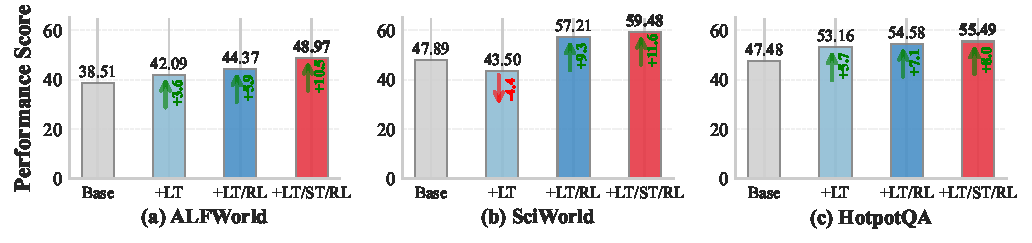
\includegraphics[width=\textwidth]{results/fig_ablation_components_qwen3.pdf}
  \caption{Ablation study results for Qwen3-4B-Instruct. 
  \textbf{Base}: No-Memory baseline; \textbf{+LT}: AgeMem-noRL-RAG (LTM tools only); 
  \textbf{+LT/RL}: AgeMem-RAG (RL with LTM tools); 
  \textbf{+LT/ST/RL}: AgeMem (full AgeMem system with RL). 
  Green arrows indicate performance gains over the baseline. }
  \label{fig:ablation_qwen3}
\end{figure*}

This section provides complementary ablation study results for Qwen3-4B-Instruct. Figure~\ref{fig:ablation_qwen3} shows the progressive contribution of LTM, STM, and RL components on Qwen3-4B-Instruct across three representative datasets. The results demonstrate consistent trends with Qwen2.5-7B-Instruct, validating the generalizability of our approach across different model sizes.

\subsection{Reward Function Ablation on Qwen3-4B}
\label{app:qwen3_results}

To validate the generalizability of our multi-component reward design across different model architectures and scales, we conduct the same reward function ablation study as in the main text on Qwen3-4B-Instruct. This section provides a complete analysis parallel to the Qwen2.5-7B-Instruct results presented in the main paper.

\subsubsection{Convergence Analysis}

\begin{figure}[t]
\centering
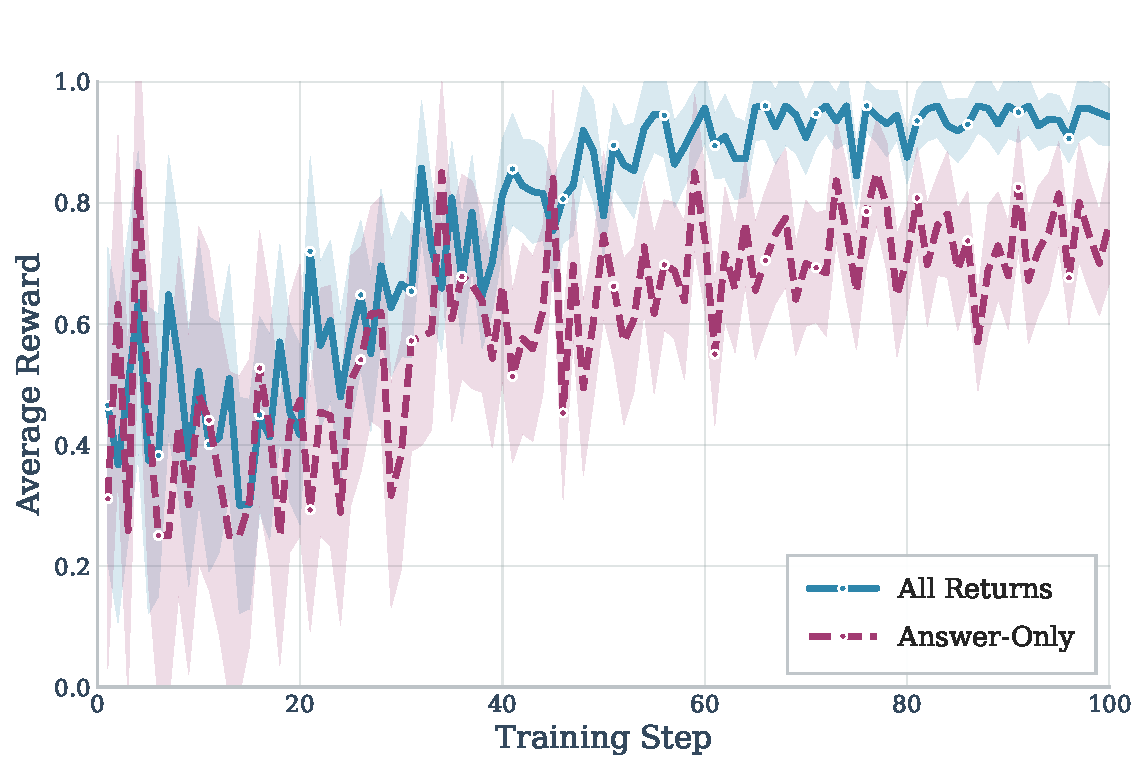
\includegraphics[width=\columnwidth]{results/qwen3_4B_reward_trends.pdf}
\caption{Training convergence curves on Qwen3-4B-Instruct comparing All-Returns (solid line) v.s. Answer-Only (dashed line) reward strategies. }
\label{fig:reward_convergence_qwen3}
\end{figure}

Figure~\ref{fig:reward_convergence_qwen3} demonstrates the reward convergence patterns on Qwen3-4B-Instruct. Similar to Qwen2.5-7B-Instruct, the All-Returns strategy consistently outperforms Answer-Only throughout the training process. Several notable observations emerge:

\textbf{More Stable Dynamics:} The convergence curve shows noticeably smoother progression with lower variance, particularly in the later training stages (steps 70-100). This stability suggests that Qwen3's architecture may have better inductive biases for the reward learning task.

\textbf{Consistent Superiority:} While the absolute improvement is smaller than Qwen2.5-7B-Instruct, the All-Returns strategy maintains its advantage throughout training, validating the robustness of our reward design.

\subsubsection{Quantitative Results}

\begin{table}[t]
\centering
\small
\caption{Reward function ablation results on HotpotQA using Qwen3-4B-Instruct. All-Returns v.s. Answer-Only reward strategies. ``TN'' is the token number, and ``TC'' denotes the number of tool calls.}
\label{tab:reward_ablation_qwen3}
\begin{tabular}{@{}lcccc@{}}
\toprule
\textbf{Strategy} & \textbf{J}($\uparrow$) & \textbf{TN}($\downarrow$) & \textbf{MQ}($\uparrow$) & \textbf{TC}(-) \\
\midrule
Answer-Only & 0.546 & \textbf{2164} & 0.415 & 7.21 \\
All-Returns & \textbf{0.555} & 2191 & \textbf{0.605} & 8.67 \\
\bottomrule
\end{tabular}
\vspace{-0.2cm}
\end{table}

Table~\ref{tab:reward_ablation_qwen3} reports the reward ablation results on HotpotQA with Qwen3-4B-Instruct. Compared to the Answer-Only strategy, the All-Returns reward consistently improves overall performance. In particular, it yields higher LLM-as-a-Judge scores (0.555 v.s. 0.546) and substantially better memory quality (MQ: 0.605 v.s. 0.415), indicating that explicitly rewarding memory-related behaviors leads to more reliable memory organization. The All-Returns strategy also encourages more active tool usage (8.67 v.s. 7.21), suggesting that the agent learns to leverage memory operations more effectively when intermediate returns are optimized. This improvement comes with only a marginal increase in token consumption (2191 v.s. 2164), implying that the gains are not driven by excessive context expansion but by more efficient memory utilization. Overall, these results show that incorporating memory-aware rewards significantly enhances both memory quality and task performance on Qwen3-4B-Instruct. The observed trends are consistent with those obtained on Qwen2.5-7B-Instruct, confirming the robustness of the reward design across different model backbones.
